% begin module arctan-ex3
\begin{frame}
\begin{example}
Simplify the expression $\cos (\tan^{-1} x)$.
\begin{itemize}
\item<2->  Let $y = \tan^{-1} x$, so $\tan y = x$.
\item<3->  Draw a right triangle with opposite $x$ and adjacent $1$.
\item<4->  \alert<handout:0| 4-5>{Length of hypotenuse $ = \uncover<5->{\sqrt{1^2+x^2}.}$}
\item<6->  Then \alert<handout:0| 6-7>{$\cos (\tan^{-1}x) = \uncover<7->{1/\sqrt{1+x^2}.}$}
\end{itemize}
\ \only<handout:0| -2>{%
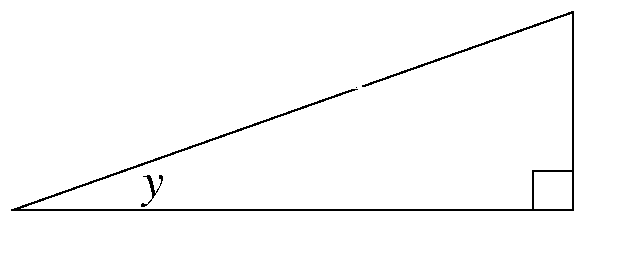
\includegraphics[width=5cm]{inverse-trig/pictures/07-06-ex3a.pdf}%
}%
\only<handout:0| 3-4>{%
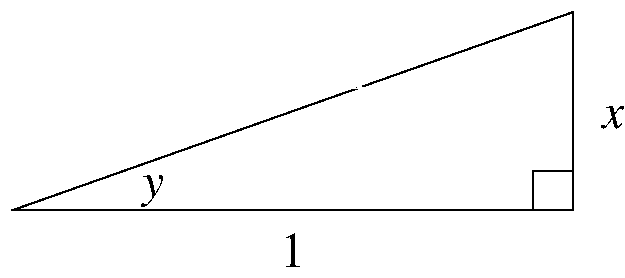
\includegraphics[width=5cm]{inverse-trig/pictures/07-06-ex3b.pdf}%
}%
\only<5->{%
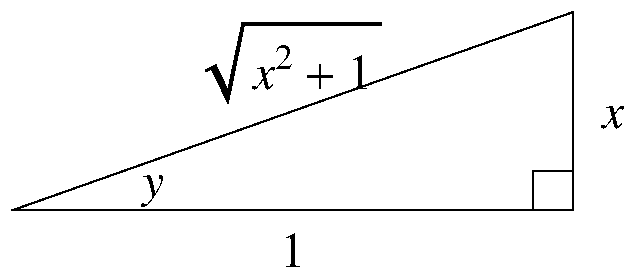
\includegraphics[width=5cm]{inverse-trig/pictures/07-06-ex3c.pdf}%
}%
\end{example}
\end{frame}
% end module arctan-ex3
